

%%%%%%%%%%%%%%%%%%%%%%%%%%%%%%%%%%%%%%%%%%%%%%%%%%%%%%%%%%%%%%%%%%%%%%
%%%%%%%%%%%%%%%%%%%%%%%%% POSTAVKE %%%%%%%%%%%%%%%%%%%%%%%%%%%%%%%%%%%
%%%%%%%%%%%%%%%%%%%%%%%%% NE MIJENJATI %%%%%%%%%%%%%%%%%%%%%%%%%%%%%%%
%%%%%%%%%%%%%%%%%%%%%%%%%%%%%%%%%%%%%%%%%%%%%%%%%%%%%%%%%%%%%%%%%%%%%%

\documentclass[12pt,oneside, a4paper]{book}

%Ovo su paketi koji se koriste za kompajliranje dokumenta
%Vecina paketa je ukljucena po defaultu u texlive 2013 i novijim verzijama
\usepackage{etex}
\usepackage{xcolor}
\usepackage[pdftex]{graphicx}
\usepackage{rotating}
\usepackage{epsfig}
\usepackage{epstopdf}
\usepackage[T1]{fontenc}
\usepackage[utf8]{inputenc}
\usepackage{cmap}
\usepackage[croatian]{babel}
\usepackage[unicode]{hyperref}
\usepackage{mathptmx}
\usepackage{amscd}
\usepackage{amssymb}
\usepackage{amsmath}
\usepackage{amsfonts}
\usepackage[left=2.5cm,right=2.5cm,top=2.5cm,bottom=2.5cm]{geometry}
\usepackage{setspace} 
\usepackage{hhline}
\usepackage{enumerate}
\usepackage{delarray}
\usepackage{array}  
\usepackage{tabularx} 
\usepackage{multirow}  
\usepackage[bf, font=small]{caption}
\usepackage[labelfont=small, font=small]{subcaption}
\usepackage{wasysym}
\usepackage{subeqnarray}
\usepackage{pdflscape} % setting page into landscape view
\usepackage{enumitem} % for itemize lists
\usepackage[toc,page]{appendix}
\newcommand{\HRule}{\rule{\linewidth}{0.5mm}}
\usepackage{makeidx}
\usepackage{nomencl}
\usepackage{listings}
\lstset{basicstyle=\ttfamily,breaklines=true}
\usepackage{courier}
% Podesavanje izgleda zaglavlja i podnozja strana
\usepackage{fancyhdr} 

\fancypagestyle{plain}{%
  \fancyhf{}% Clear header/footer
  \fancyfoot[OR]{{\thepage}}%
  \fancyfoot[EL]{{\thepage}}%
  \renewcommand{\headrulewidth}{0pt}%
}

% required for printing index
% use \index{name} in text
%\usepackage{makeidx}S
%\makeindex
% required for printing nomenclature
% use \nomenclature{symbol}{description} in text
%\usepackage{nomencl}
%\makenomenclature
%\renewcommand{\nomname}{Popis oznaka}


%Opcionalno
%\linespread{1.3}
%\setlist{nolistsep}   % setting for itemize lists
%\renewcommand{\thefootnote}{\fnsymbol{footnote}}  % to get unnumbered footnotes

% Adding a dot after chapter number in TOC 
%\let\savenumberline\numberline
%\def\numberline#1{\savenumberline{#1.}}

%\pagestyle{fancyplain}

%\rfoot{\thepage}
% iskljucivanje broja strane iz Sadrzaja, Popisa slika i Popisa tabela
\AtBeginDocument{\addtocontents{toc}{\protect\thispagestyle{empty}}}
\AtBeginDocument{\addtocontents{lof}{\protect\thispagestyle{empty}}}
\AtBeginDocument{\addtocontents{lot}{\protect\thispagestyle{empty}}}

%\rhead{\slshape \nouppercase \leftmark}
%\lhead{} %delete left header


%Podesavanje izgleda referenci
\usepackage[square, numbers, sort]{natbib} 

%Promjena naziva pojedinih poglavlja sa Hrvatskog na Bosanski
% Bibliography u "Literatura"
\addto\captionscroatian{%
  \renewcommand{\bibname}{Literatura}
  \renewcommand{\tablename}{Tabela}
  \renewcommand{\nomname}{Popis oznaka}
  \renewcommand{\indexname}{Indeks pojmova}
  \renewcommand{\lstlistingname}{Program}
}
%"Popis tablica" u "Popis tabela"
\addto\captionscroatian{\renewcommand{\listtablename}{Popis tabela}}
\addto\captionscroatian{\renewcommand\appendixname{Prilog}}
\addto\captionscroatian{\renewcommand\appendixpagename{Prilozi}}
\renewcommand\appendixtocname{Prilozi}

\makeindex
\makenomenclature

%\usepackage{etoolbox}
%\patchcmd{\chapter}{\thispagestyle{plain}}{\thispagestyle{fancyplain}}{}{}


\begin{document}

%%%%%%%%%%%%%%%%%%%%%%%%%%%%%%%%%%%%%%%%%%%%%%%%%%%%%%%%%%%%%%%%%%%%%%
%%%%%%%%%%%%%%%%%%%%%%%%% OSNOVNI DOKUMENT %%%%%%%%%%%%%%%%%%%%%%%%%%%
%%%%%%%%%%%%%%%%%%%%%%%%%%%%%%%%%%%%%%%%%%%%%%%%%%%%%%%%%%%%%%%%%%%%%%

\frontmatter

%%%%%%%%%%%%%%%%%%%% NASLOVNA STRANA %%%%%%%%%%%%%%%%%%%%%%%%
\begin{titlepage}
\begin{center}


\includegraphics[width=0.25\textwidth]{etf-logo.png}~\\[0.1cm]
\textsc{\Large Univerzitet u Sarajevu}\\[0.2cm]  
\textsc{\Large Elektrotehnički fakultet}\\[0.2cm] 
\textsc{\Large Odsjek za racunarstvo i informatiku }\\[3cm]\HRule \\[0.5cm] 
{\huge \bfseries Prostorna analiza u NoSQL bazama podataka} \\[0.4cm] 
\HRule \\[0.5cm]

\textsc{\Large Završni rad}\\[0.4cm]
\textsc{\Large - Prvi ciklus studija - }\\[1.5cm]

% Author and supervisor 
\textbf{ 
\Large Student:\\  
\Large Kenan Abadzic\\[1cm]  
\Large Mentor: \\[0.2cm] 
\Large Red.prof.dr. Almir Karabegović\\[0.2cm]} 
\vfill

% Bottom of the page  
{\large Sarajevo, juli 2025.}

\end{center} 
\end{titlepage}

% Sažetak (na Bosanskom jeziku) i Abstract (na Engleskom jeziku),
% postavka rada i izjava o autentičnoati su dati kao odvojeni fajlovi

%%%%%%%%%%%%%% SAŽETAK I ABSTRACT %%%%%%%%%%%%%%%%%%%%%%%%%%%%%%%%
\pagebreak

\section*{Sažetak}


Ovo je \LaTeX\ predložak za izradu završnog rada prvog ciklusa studija, izrađen za potrebe studenata Elektrotehničkog fakulteta u Sarajevu. U radu se isprepliću dvije odvojene cjeline - sadržaj i forma. Sadržaj rada je baziran na idejama iz važećeg Pravilnika o strukturi i sadržaju doktorske disertacije i magistarskog rada na Elektrotehničkom fakultetu u Sarajevu (br. 04-1-673/11, dana 17.01.2011. godine), dok je forma rada definirana strukturom i načinom korištenja .tex fajlova.
U fajlu Zavrsni\_rad\_BSc\_Ime\_Prezime.tex oblikovane su osnovne stranice, a naredbom \textit{include} umeću se dodatne stranice i dodaju poglavlja. 

Osim \textit{Zavrsni\_rad\_BSc\_Ime\_Prezime.tex} fajla, koristi se još i: \textit{abstract.tex} (izdvojen fajl za sažetak na bosanskom i engleskom jeziku), \textit{postavka.tex} (izdvojen fajl za postavku rada), \textit{izjava.tex} (izdvojen fajl za izjavu o autentičnosti rada), \textit{poglavlje\_1.tex} (primjer jednog poglavlja),\textit{ prilog\_1.tex} (primjer jednog priloga) i \textit{literatura.bib} (bibliografski podaci).

U sažetku je potrebno dati koncizan opis riješenih problema, metoda korištenih za njegovo (njihovo) rješavanje, dobivenih rezultata i zaključke. U sažetku se ne navode reference. Potrebno je voditi računa da se u sažetku ne daje uvod u rad, niti pregled poglavlja rada, već daje opis namjene rada do najviše 500 riječi.

\vspace{1cm}
\textbf{Ključne riječi}:  predložak, \LaTeX, ETF

\section*{Abstract}

The section "Sažetak" should actually be translated to the section "Abstract". Please avoid the direct usage of google-translate.  

\vspace{1cm}
\textbf{Keywords}:  template, \LaTeX , ETF

%%%%%%%%%%%%%%%%%%%% POSTAVKA RADA %%%%%%%%%%%%%%%%%%%%%%%%%%%%%%%
%%%%%%%%%%%%%%%%%%%% POSTAVKA RADA %%%%%%%%%%%%%%%%%%%%%%%%%%%%%%%
\thispagestyle{plain}
\begin{flushleft}
\textbf{Elektrotehnički fakultet, Univerzitet u Sarajevu}\\
\textbf{Odsjek za ..............}\\
\textbf{Vanr. prof. dr Alessandro Volta, dipl.el.ing}\\


\textbf{Sarajevo, .........(datum) }\\
\end{flushleft}

\begin{center}
\vspace{2cm}
{\Large Postavka zadatka završnog rada I ciklusa:}\\
\vspace{0.2cm}
{\large \textbf{Predložak za izradu završnog rada I ciklusa - uz korištenje Latexa kao alata}}
\end{center}

\vspace{0.5cm}
U okviru rada je potrebno razviti \LaTeX\ predložak za izradu završnog rada prvog ciklusa studija. U radu je potrebno:
\begin{itemize}
\item objasniti opći postupak za izradu i pisanje završnih radova prvog ciklusa studija, poštivajući odgovarajuće Pravilnike,
\item dati kratko uputstvo za korištenje .tex dokumenata, pisanje slika, tabela i relacija, generisanje sadržaja, popisa slika i tabela i sl.
\item dati kratko upusto za generiranje odgovarajućih .pdf dokumenata iz odgovarajućih .tex fajlova,
\end{itemize}
Preporučuje se korištenje TexLive \LaTeX\ podrške, verzije 2013 ili novije.

\textbf{Napomena: U dijelu "Postavka" se stavlja postavka rada koju je specificirao mentor prilikom davanja teme. Naročito obratiti pažnju na naslov rada koji mora biti konzistentan tokom cijelog dokumenta, i usaglašen sa temom upisanom u informacioni sistem (npr. Zamger). Na ovoj stranici se potpisuje mentor prije nego se radovi odnesu u studentsku službu.}


\vspace{1cm}
\textbf{Polazna literatura:}

\begin{itemize}
\item[]  [1] Sonka, M., Hlavec, V., Boyle, R., "Image Processing, Analysis, and Machine Vision", Thomson, 2008.
\item[] [2] Lee, E.A., Varaiya, P., "Structure and Interpretation of Signals and Systems", Electrical Engineering \& Computer Science University of California, Berkeley, 2000

\end{itemize}


\begin{center}
\vspace{2cm}
\makebox[8cm]{\hrulefill} \\
Vanr. prof. dr Alessandro Volta, dipl. ing. el.\\
\end{center}







%%%%%%%%%%%%%%%%%%%% IZJAVA AUTORA %%%%%%%%%%%%%%%%%%%%
%%%%%%%%%%%%%%%%%%%% IZJAVA AUTORA %%%%%%%%%%%%%%%%%%%%

%\chapter*{Izjava autora}
\pagebreak

\thispagestyle{plain}
\begin{flushleft}
	\textbf{Univerzitet u Sarajevu}\\
	\textbf{Elektrotehnički fakultet}\\
	\textbf{Odsjek za ............ }\\
\end{flushleft}

\begin{center}
	\vspace{1cm}
	{\Large \textbf{Izjava o autentičnosti radova}}\\
	\vspace{0.3cm}
	{\Large Završni rad}\\
	\vspace{0.2cm}
	{\Large I ciklusa studija}
	\vspace{0.5cm}
\end{center}

\noindent{Ime i prezime:  ............ }\\
\noindent{Naslov rada:  ............ }\\
\noindent{Vrsta rada: Završni rad  Prvog ciklusa studija}\\
\noindent{Broj stranica:  ............ \\
\vspace{0.5cm}

\noindent\textbf{\large Potvrđujem:}
%\vspace{0.2cm}
\begin{itemize}
	\item da sam pročitao dokumente koji se odnose na plagijarizam, kako je to definirano Statutom Univerziteta u Sarajevu, Etičkim kodeksom Univerziteta u Sarajevu i pravilima studiranja koja se odnose na I i II ciklus studija, integrirani studijski program I i II ciklusa i III ciklus studija na Univerzitetu u Sarajevu, kao i uputama o plagijarizmu navedenim na web stranici Univerziteta u Sarajevu;
	\item da sam svjestan univerzitetskih disciplinskih pravila koja se tiču plagijarizma;
	\item da je rad koji predajem potpuno moj, samostalni rad, osim u dijelovima gdje je to naznačeno;
	\item da rad nije predat, u cjelini ili djelimično, za stjecanje zvanja na Univerzitetu u Sarajevu ili nekoj drugoj visokoškolskoj ustanovi;
	\item da sam jasno naznačio prisustvo citiranog ili parafraziranog materijala i da sam se referirao na sve izvore;
	\item da sam dosljedno naveo korištene i citirane izvore ili bibliografiju po nekom od preporučenih stilova citiranja, sa navođenjem potpune reference koja obuhvata potpuni bibliografski opis korištenog i citiranog izvora;
	\item da sam odgovarajuće naznačio svaku pomoć koju sam dobio pored pomoći mentora i akademskih tutora/ica.
\end{itemize}
\vspace{0.5cm}
\noindent {Sarajevo, datum  ....... }
\begin{center}
	\vspace{1.5cm}
	Potpis:\\
	\vspace{0.5cm}
	\makebox[8cm]{\hrulefill} \\
	 (ime) .........\\
\end{center}
\clearpage


%%%%%%%%%%%%%%%%%%%%% SADRŽAJ %%%%%%%%%%%%%%%%%%%%%%%%%
\clearpage
\tableofcontents

%%%%%%%%%%%%%%% POPIS SLIKA %%%%%%%%%%%%%%%%%%%%%%%%%%%
%\clearpage
\listoffigures
\addcontentsline{toc}{chapter}{Popis slika}

%%%%%%%%%%%%%%% POPIS TABELA %%%%%%%%%%%%%%%%%%%%%%%%%%
%\clearpage
\listoftables
\addcontentsline{toc}{chapter}{Popis tabela}

%%%%%%%%%%%%%%% POPIS OZNAKA %%%%%%%%%%%%%%%%%%%%%%%%%%%
\cleardoublepage % start new page
\pagestyle{fancyplain} % puts headers/footers back on
\fancyhf{}
\lhead{\nouppercase{\fancyplain{}{\leftmark}}}
\renewcommand{\chaptermark}[1]{\markboth{#1}{}}
\renewcommand{\footrulewidth}{0.4pt} %draw foot line
\lfoot{\slshape Tesla, N., "Predložak za izradu završnog rada"}
\rfoot{\thepage}
\cfoot{}

%%%%%%%%%%%%%%%%%%%%%%%%%%%%%%%%%%%%%%%%%%%%%%%%%%%%%%%%%%%%%%%%%%%%
\mainmatter

%%%%%%%%%%%%%%%%%%%%%%%%%%%%%%%%%%%%%%%%%%%%%%%%%%%%%%%%%%%%%%%%%%%%
%%%%%%%%%%%%%%%%%%%%%%%%% POGLAVLJA %%%%%%%%%%%%%%%%%%%%%%%%%%%%%%%%
%%%%%%%%%%%%%%%%%%%%%%%%%%%%%%%%%%%%%%%%%%%%%%%%%%%%%%%%%%%%%%%%%%%%

%Poglavlja je najbolje raditi u odvojenim fajlovima
%Uvod
\chapter{Uvod}

U skladu sa dobrom istraživačkom praksom, uvodno poglavlje rada prvog ciklusa studija bi trebao sadržavati bar sljedeće elemente: 
\begin{itemize}
\item {obrazloženje teme,}
\item {opis strukture rada.}
\end{itemize}

U narednom tekstu će detaljnije biti obrazložena svaka od tačaka.

\section{Obrazloženje teme}
U ovoj sekciji autor je dužan da obrazloži koja tema ili problem će biti analizirani ili istraživani, te zbog čega je upravo ova tema pogodna i bitna za istraživanje. Pohvalno je napraviti pregled literature sa odgovarajućim referenciranjem na istu.

\section{Struktura rada}
U ovoj sekciji je najbolje dati po jedan paragraf o svakom poglavlju iz rada. Potencirajte koji su glavni doprinosi svakog poglavlja, te kako su poglavlja medjusobno povezana.





%Teorijski okviri
\chapter{Teorijski okviri}

Istraživanje se izlaže organizirano, koncizno i konzistentno kroz dva ili više odvojenih poglavlja, sa  pregledom teoretskih osnova na kojima su bazirana i kraćom diskusijom dobijenih rezultata. Ono što je izuzetno važno jeste da se dobiveni rezultati istraživanja konstantno objektivno porede sa postojećim rezultatima u literaturi ili oblasti istraživanja, te sistematično ukazuje na prednosti i nedostatke autorskog pristupa.
Izostanak komparacije rezultata istraživanja dobivenih od strane autora sa konkurentnim algoritmima, metodama i pristupima pokazuje nepostojanje akademske zrelosti, nedovoljnu posvećenost u istraživanju odgovarajuće naučne oblasti i vrlo često ukazuje na loš kvalitet disertacije/rada.

U radu se za formiranje poglavlja koriste sekcije, podsekcije, podpodsekcije, paragrafi i podparagrafi kao u primjerima koji slijedi.
 
\section{Primjer sekcije}
Ovo je primjer sekcije. Ovo je primjer sekcije. Ovo je primjer sekcije. Ovo je primjer sekcije. Ovo je primjer sekcije. Ovo je primjer sekcije. Ovo je primjer sekcije. Ovo je primjer sekcije. Ovo je primjer sekcije. Ovo je primjer sekcije. Ovo je primjer sekcije. Ovo je primjer sekcije. Ovo je primjer sekcije. Ovo je primjer sekcije. Ovo je primjer sekcije. Ovo je primjer sekcije. Ovo je primjer sekcije.
\subsection{Primjer podsekcije}
Ovo je primjer podsekcije. Ovo je primjer podsekcije. Ovo je primjer podsekcije. Ovo je primjer podsekcije. Ovo je primjer podsekcije. Ovo je primjer podsekcije. Ovo je primjer podsekcije. Ovo je primjer podsekcije. Ovo je primjer podsekcije. Ovo je primjer podsekcije. Ovo je primjer podsekcije. Ovo je primjer podsekcije. Ovo je primjer podsekcije. Ovo je primjer podsekcije. Ovo je primjer podsekcije.
\subsubsection{Primjer podpodsekcije}
Ovo je primjer podpodsekcije. Ovo je primjer podpodsekcije. Ovo je primjer podpodsekcije. Ovo je primjer podpodsekcije. Ovo je primjer podpodsekcije. Ovo je primjer podpodsekcije. Ovo je primjer podpodsekcije. Ovo je primjer podpodsekcije. Ovo je primjer podpodsekcije. Ovo je primjer podpodsekcije. Ovo je primjer podpodsekcije. Ovo je primjer podpodsekcije. Ovo je primjer podpodsekcije.
\paragraph{Primjer paragrafa}
Ovo je primjer paragrafa. Ovo je primjer paragrafa. Ovo je primjer paragrafa. Ovo je primjer paragrafa. Ovo je primjer paragrafa. Ovo je primjer paragrafa. Ovo je primjer paragrafa. Ovo je primjer paragrafa. Ovo je primjer paragrafa. Ovo je primjer paragrafa. Ovo je primjer paragrafa. Ovo je primjer paragrafa. Ovo je primjer paragrafa. Ovo je primjer paragrafa.
\subparagraph{Primjer podparagrafa}
Ovo je primjer podparagrafa. Ovo je primjer podparagrafa. Ovo je primjer podparagrafa. Ovo je primjer podparagrafa. Ovo je primjer podparagrafa. Ovo je primjer podparagrafa. Ovo je primjer podparagrafa. Ovo je primjer podparagrafa. Ovo je primjer podparagrafa. Ovo je primjer podparagrafa. Ovo je primjer podparagrafa. Ovo je primjer podparagrafa. Ovo je primjer podparagrafa. Ovo je primjer podparagrafa.

\begin{center}
\vspace{0.5cm}
*\hspace{2cm}*\hspace{2cm}*
\vspace{0.3cm}
\end{center}

Na kraju svakog poglavlja, najbolje je dati jedan kraći zaključak koji ukratko objedinjuje sve najvažnije zaključke iz tog poglavlja. Taj kraći zaključak treba da služi kao poveznica između poglavlja koje se upravo završilo, i narednog poglavlja koje tek treba da počne. Ovaj zaključak je poželjno odvojiti bilo kao odvojenu podsekciju poglavlja nazvanu "Zaključak", bilo kao jednostavno izdvojeni dio teksta razmaknut zvjezdicama.

Kratak primjer zaključka za ovo poglavlje: U ovom poglavlju je pokazano kako se formiraju centralna poglavlja u radu/disertaciji. U nastavku će biti pokazano kako se piše konačan zaključak, te dati određeni tehnički podaci oko formatiranja teksta, slika i formula.


%Pregled stanja
\chapter{Pregled stanja u obradi prostornih podataka u NoSQL bazama podataka}
\section{Uvod}  
Istraživanje se izlaže organizirano, koncizno i konzistentno kroz dva ili više odvojenih poglavlja, sa  pregledom teoretskih osnova na kojima su bazirana i kraćom diskusijom dobijenih rezultata. Ono što je izuzetno važno jeste da se dobiveni rezultati istraživanja konstantno objektivno porede sa postojećim rezultatima u literaturi ili oblasti istraživanja, te sistematično ukazuje na prednosti i nedostatke autorskog pristupa.
%Primjer implementacije s MongoDB bazom podataka
\chapter{Primjer implementacije s MongoDB bazom podataka}

\section{Primjer sekcije}
Ovo je primjer sekcije. Ovo je primjer sekcije. Ovo je primjer sekcije. Ovo je primjer sekcije. Ovo je primjer sekcije. Ovo je primjer sekcije. Ovo je primjer sekcije. Ovo je primjer sekcije. Ovo je primjer sekcije. Ovo je primjer sekcije. Ovo je primjer sekcije. Ovo je primjer sekcije. Ovo je primjer sekcije. Ovo je primjer sekcije. Ovo je primjer sekcije. Ovo je primjer sekcije. Ovo je primjer sekcije.
%Analiza rezultata
\chapter{Rezultati i diskusija}
Istraživanje se izlaže organizirano, koncizno i konzistentno kroz dva ili više odvojenih poglavlja, sa  pregledom teoretskih osnova na kojima su bazirana i kraćom diskusijom dobijenih rezultata. Ono što je izuzetno važno jeste da se dobiveni rezultati istraživanja konstantno objektivno porede sa postojećim rezultatima u literaturi ili oblasti istraživanja, te sistematično ukazuje na prednosti i nedostatke autorskog pristupa.
%Zaključak
\chapter*{Zaključak}

Preporučuje se da se poglavlje "Uvod" i "Zaključak", te odgovarajuće sekcije i podsekcije ne numerišu. Ovo poglavlje bi trebalo na izvjestan način objediniti sve "kraće" zaključke date na kraju pojedinih poglavlja.

\section*{Ostvareni ciljevi završnog rada}

U ovoj sekciji je potrebno dati jasan sumarni pregled obavljenih istraživanja i dobijenih rezultata. Rezultati trebaju biti struktuirani i prikazani prema okvirima i ciljevima postavljenim u uvodnom poglavlju.
Potrebno je i provesti poredjenja dobivenih rezultata sa literaturom navedenom u uvodnom poglavlju, te dati diskusiju kako se dobijeni rezultati uklapaju, potvrdjuju, nadopunjuju ili su kontradiktorni onim koji su prikazani u uvodnom poglavlju. 




%%%%%%%%%%%%%%%%%%%%% PRILOZI %%%%%%%%%%%%%%%%%%%%%%%%%%%%%%%%%%%%
\begin{appendices}
%Priloge je najbolje raditi u odvojenim fajlovima
%Prilog 1
\chapter{Korištenje funkcija u Tex-u}

Sadržaji koji se mogu uključiti u Priloge su: izvođenje jednačina i formula, detalji važnijih softverskih programa, razne tabele i dijagrami, karkateristike i performanse ili opisi opreme i komponenti koje su korištene u disertaciji/radu. Mogu se takodjer uključiti konstrukcioni crteži ili električne sheme.

U ovom prilogu prikazane su neke od funkcije koje se mogu koristiti prilikom oblikovanja rada i prikaza rezultata istraživanja korištenjem \LaTeX a. 


\section{Matematički izraz}


Primjer matematičke formule prikazan je izrazom

\begin{equation}
  T: \mathbf{x}_B \mapsto \mathbf{x}_A \Leftrightarrow T(\mathbf{x}_B) = \mathbf{x}_A.
  \label{eq:transformacija}
\end{equation}

Matematičke relacije se u \LaTeX razvojnom okruženju automatski numeriraju. Međutim, da bi se pojedina relacija (slika, tabela) referencirala u tekstu, potrebno je da se svakoj relaciji (slici, tabeli) dodijeli pogodna labela npr. {\tt {\textbackslash label\{MojaRelacija\}}}, a potom referencira u .tex fajlu sa {\tt {\textbackslash ref\{MojaRelacija\}}}. Na taj način će se \LaTeX pobrinuti za odgovarajuće kros-referenciranje.

\section{Slika}
Slika \ref{fig:Slika_citat} služi kao primjer uključivanja slike \index{uključivanje slike} u tekst. Relacije, slike i tabele se automatski numeriraju u \LaTeX u, i to sa oznakom brojpoglavlja.brojslike (npr. u Poglavlju 3 se numeriraju sa 3.1, 3.2, ... neovisno od toga u kojoj sekciji ili podsekciji se nalaze).

\begin{figure}
  \centering
  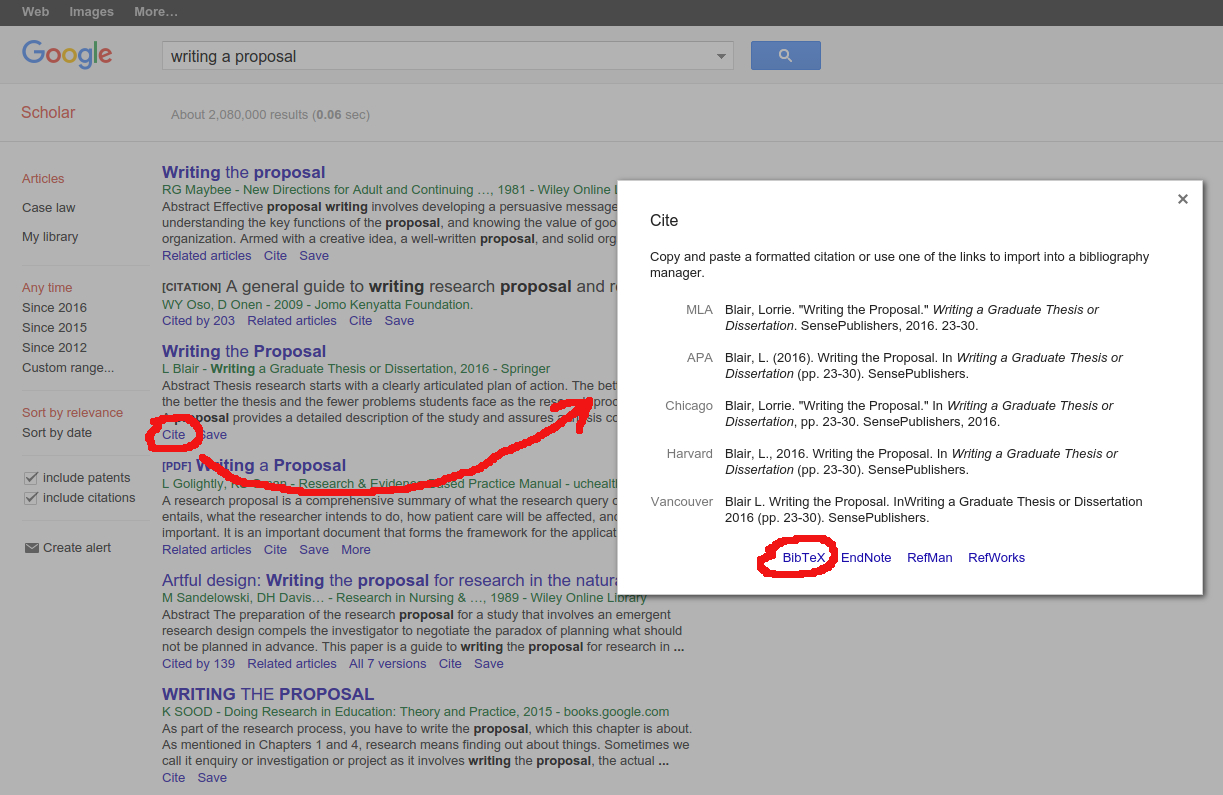
\includegraphics[width=0.7\textwidth]{SlikaCitat}
  \caption{Primjer naslova slike - uputstvo za traženje bibiografskih referenci na Google Scholar.}
  \label{fig:Slika_citat}
\end{figure}

\begin{figure}
  \centering
  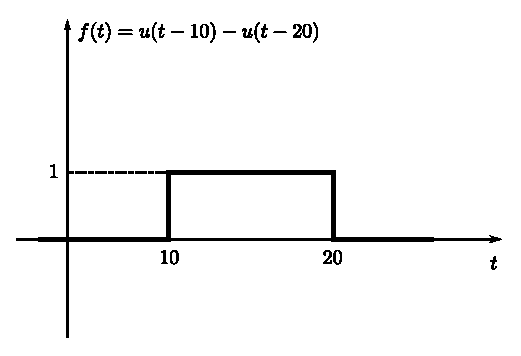
\includegraphics[width=0.5\textwidth]{SlikaCitat3}
  \caption{Primjer dijagrama - veličina i tip fonta na slici bi trebao odgovarati veličini i tipu fonta u tekstu}
  \label{fig:Slika_citat_3}
\end{figure}


\section{Tabela}
Formiranje tabele prikazano je na primjeru u Tabeli \ref{tab:confusion_matrix}. Za razliku od naslova slika, naslov tabela stoji iznad odgovarajućih tabela u tekstu.
\renewcommand{\arraystretch}{1.5} % prosirivanje redova u tabeli
\begin{table} [!ht]
  \caption{Naslov tabele}
  \begin{center}
  \begin{tabular}{ | c | c | c | c |}
	\hline
    Oznaka reda & Kolona 1 & Kolona 2 & Kolona 3 \\
    \hline 
    \hline
    red 1 & 1 & 2 & 3 \\ 
    \hline
    red 2 & 3 & 2 & 1 \\ 
     \hline
    red 3 & $E=mc^2$ & 2 & 3 \\ 
     \hline
  \end{tabular}
  \label{tab:confusion_matrix}    
\end{center} 
\end{table}
\renewcommand{\arraystretch}{1} % vraćeno na staro

\section{\textit{Landscape}}

Postavljanja stranice u prikaz \textit{landscape} prikazano je umetanjem izduzene Slike \ref{fig:Slika_citat2} u \textit{landscape} format papira. 

\begin{landscape}
 \begin{figure}
  \centering
  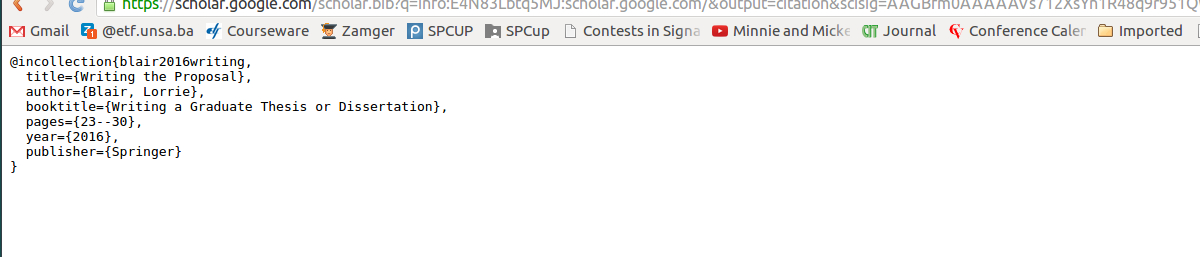
\includegraphics[width=25cm]{SlikaCitat2}
  \caption{Primjer ekstrakcije bibliografskih stavki za kopiranje u .bib fajl, sa Google Scholara}
  \label{fig:Slika_citat2}
\end{figure}
\end{landscape}

\section{Indeks pojmova i Popis oznaka}

Ukoliko je u radu neophodno uvesti i indeks, odnosno popis oznaka, onda se to radi na sljedeći način. Prilikom definiranja indeksa koristi se {\tt \textbackslash index\{ime\}}. Npr. {\tt \textbackslash index\{uključivanja slike\}}. 

Kod dodavanja pojmova u Popis oznaka u .tex fajlu se koristi {\tt \textbackslash nomenclature\{simbol\} \{opis\}}, npr. {\tt \textbackslash nomenclature\{ETF\}\{Elektrotehnički fakultet\}}.
Generiranje indeksa i Popisa oznaka se pravi korištenjem naredbi {\tt \textbackslash makeindex} i {\tt \textbackslash makenomenclature} u preambli, odnosno {\tt \textbackslash printindex} i {\tt \textbackslash printnomenclature} na mjestu generiranja popisa. 
Osim toga, potrebno je i kompajlirati dokument sa MakeIndex. 




\section{Korištenje literature}

Popis literature navodi se na kraju rada. Da bi uz \LaTeX  efikasno koristila literatura, potrebno je da se generira fajl sa bibliografskim jedinicama. Fajl {\tt literatura.bib} je sastavni dio ovog rada, i može poslužiti kao primjer kako se pišu pojedine bibliografske jedinice. Svaki unos (referenca) sadrži labelu na tu referencu, putem koje se bilo gdje u radu može citirati npr. sa {\tt \textbackslash cite\{Hajn01\} }. 

Dobar trik za popunjavanje bibliografskih unosa u .bib fajlu je korištenje Google Scholara \url{https://scholar.google.com/}. Osim što je baza naučnih radova, Google Scholar omogućava i kopiranje zapisa referenci na ispravan način. Podržani su svi najpopularniji formati citiranja (MLA, Chicago, Harvard itd.), kao što se vidi na Slici \ref{fig:Slika_citat}. Osim toga, klikom na dugme "BibTeX", moguće je izabrati i zapis reference razumljive razvojnom okruženju \LaTeX, a nakon toga je jednostavno kopirati u bibliografski fajl  {\tt literatura.bib} (vidjeti Sliku \ref{fig:Slika_citat2}).

Primjeri navođenja literature su knjiga \cite{Hajn01}, poglavlje u knjizi \cite{Samp05}, članak objavljen u časopisu \cite{Sim03}, članak objavljen na konferenciji \cite{Wirt99}, doktorski rad \cite{Will93}, Internetski izvor \cite{Jone12} te različite druge publikacije \cite{Rsoft}. Stil navođenja literature temelji se na stilu razvijenom za IEEE časopise i konferencije.

\section{Programski kodovi}

Programski kodovi se \LaTeX u navode korištenjem okruženja {\tt lstlisting}. Primjer koda je dat ispod.

\begin{lstlisting}[frame=single,language=C++,numbers=left, numberstyle=\tiny, xleftmargin=0.05\textwidth, xrightmargin=0.05\textwidth, basicstyle=\ttfamily\footnotesize, caption=Primjer programa]
// program u C++
#include <iostream>

int main ()
{
  std::cout << "Dobar Dan! ";
  std::cout << "Prvi program u C++";
}
\end{lstlisting}

\end{appendices}

%%%%%%%%%%%%%%%%%%%%%%%%%%%%%%%%%%%%%%%%%%%%%%%%%%%%%%%%%%%%%%%%%%%
\backmatter

%%%%%%%%%%%%%%%%%%%%%%% LITERATURA %%%%%%%%%%%%%%%%%%%%%%%%%%%%%%%%%
\addcontentsline{toc}{chapter}{Literatura}
\bibliographystyle{IEEEtranETF} 
\bibliography{literatura}

%%%%%%%%%%%%%%%%%%% INDEKS POJMOVA %%%%%%%%%%%%%%%%%%%%%%%%%%%%%%%%
\addcontentsline{toc}{chapter}{Indeks pojmova}
\printindex 


\end{document}
